\documentclass[11pt,xcolor=svgnames]{beamer}
\usepackage{dsfont,natbib,setspace,changepage,multirow}
\mode<presentation>

% replaces beamer foot with simple page number
\setbeamertemplate{navigation symbols}{}
\setbeamerfont{frametitle}{series=\bfseries,size=\normalsize}
\setbeamercolor{frametitle}{fg=Black}

\setbeamertemplate{footline}{
   \raisebox{5pt}{\makebox[\paperwidth]{\hfill\makebox[20pt]{\color{gray}\scriptsize\insertframenumber}}}}

\usepackage{algorithm}
\usepackage{algorithmic}

% colors
\newcommand{\theme}{\color{Maroon}}
\newcommand{\bk}{\color{black}}
\newcommand{\rd}{\color{DarkRed}}
\newcommand{\fg}{\color{ForestGreen}}
\newcommand{\bl}{\color{blue}}
\newcommand{\gr}{\color{black!50}}
\newcommand{\sg}{\color{DarkSlateGray}}
\newcommand{\nv}{\color{Navy}}
\setbeamercolor{itemize item}{fg=gray}

% common math markups
\newcommand{\bs}[1]{\boldsymbol{#1}}
\newcommand{\mc}[1]{\mathcal{#1}}
\newcommand{\mr}[1]{\mathrm{#1}}
\newcommand{\bm}[1]{\mathbf{#1}}
\newcommand{\ds}[1]{\mathds{#1}}
\newcommand{\indep}{\perp\!\!\!\perp}
\def\plus{\texttt{+}}
\def\minus{\texttt{-}}

% spacing and style shorthand
\setstretch{1.1}

\begin{document}

\setcounter{page}{0}
{ \usebackgroundtemplate{
\includegraphics[height=\paperheight]{phoenix}}
\begin{frame}[plain]
\begin{center}

{\bf \LARGE \theme }

{\bf \Large  Making Decisions in High Dimensions}

\vskip 2cm
Matt Taddy,  Chicago Booth


\vskip .25cm
{\texttt{faculty.chicagobooth.edu/matt.taddy/research}}

\end{center}
\end{frame} }


\begin{frame}

{\bf High Dimensional Decisions}

\vskip .5cm
One of the ways that data is `Big' is in the {\theme number of inputs}.

\vskip .25cm
This number often {\theme grows with the sample size} (e.g., words in text, websites in browsers) and you never reach a statistically safe place.

\vskip .5cm
For this type of Big, we need {\nv dimension reduction} techniques: project from the full input set down to a useful low-D summary.

\vskip .25cm
Crucially, this must be focused on the {\nv decisions} you'd like to make.

\end{frame}


\begin{frame}

{\bf Fancy plot: \bk monthly stock returns}

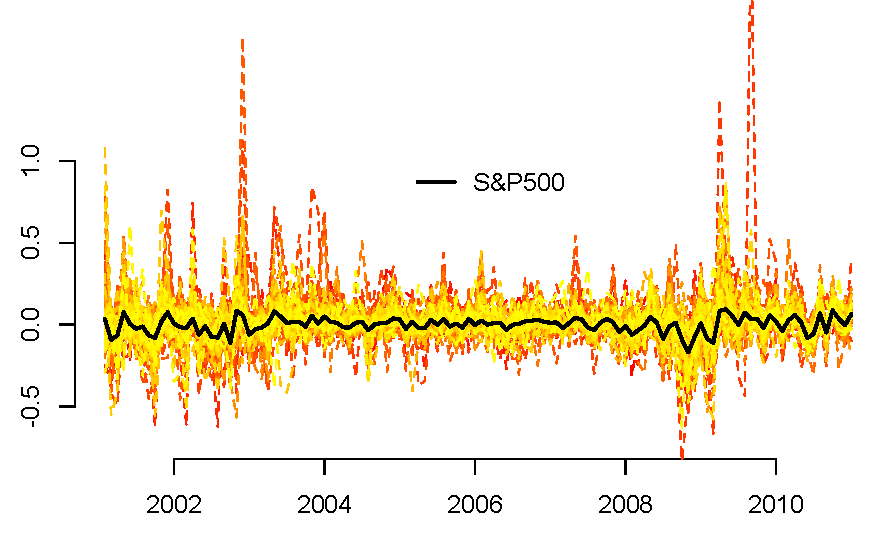
\includegraphics[width=4.25in]{graphs/fancyret}

\vskip .25cm
\hfill{\nv What do we learn?}

\vskip -.5cm
\end{frame}



\begin{frame}

{\bf Useful plot: \bk market model coefficients}

\vskip .25cm
Fit a line between stock returns $R_t$ and market returns $M_t$ (SP).
\[
R_t \approx \alpha + \beta M_t
\]
$\alpha$ is money you make regardless of what the market does.\\
$\beta$ is the asset's sensitivity to broad market movements.

\begin{center}
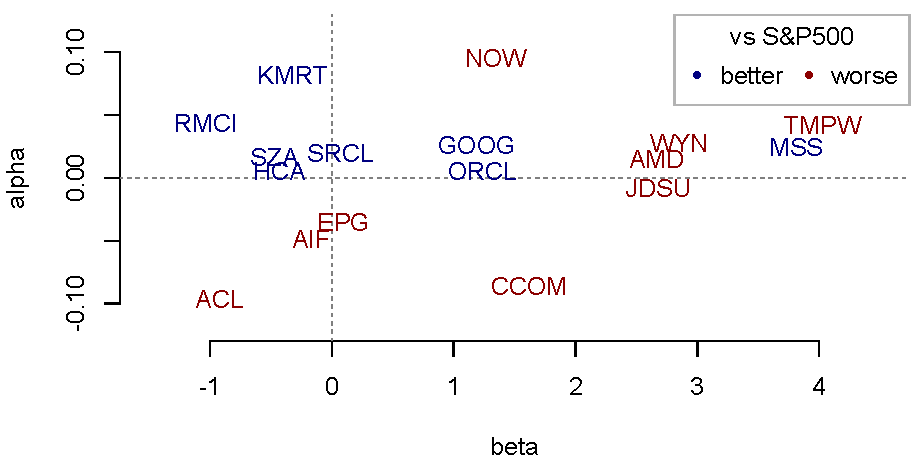
\includegraphics[width=3.5in]{graphs/usefulret}
\end{center}
\vskip -1cm
\end{frame}



\begin{frame}

Many problems in BD involve a response of interest
(`{\theme y}')\\ and a set of covariates (`{\theme \bf x}') to
be used for prediction.

\vskip .5cm
If your `decision' is to predict $y$ for new $\bm{x}$,  we need to {\nv reduce dimension} in the direction of $y$.  That is, we want to map $\bm{x}\rightarrow \hat y$.

\vskip .5cm
A general tactic is to deal in averages and lines.  \\
{We'll model the 
  conditional mean for y given {\bf x},}
\[\large
\ds{E}[~ y \mid \bm{x} ~] = f( \bm{x}'\bs{\beta} )
\]

$\bm{x} = [1, x_1, x_2,\ldots x_p]$  is your vector of
    covariates.\\
\vskip .2cm
$ \bs{\beta} = [\beta_0, \beta_1, \beta_2, \ldots \beta_p]$ are the corresponding
coefficients.

\end{frame}


\begin{frame}

{\bf Some basic facts about linear models}

\vskip .5cm
{The model is always $\ds{E}[y|\bm{x}] = f(\bm{x}\bs{\beta})$.}
\begin{itemize}
\item Gaussian (linear): $y \sim \mr{N}(\bm{x}\bs{\beta},\sigma^2)$. 
\item Binomial (logistic): $\mr{p}(y=1)= e^{\bm{x}\bs{\beta}}/(1+ e^{\bm{x}\bs{\beta}})$.
\end{itemize}

\vskip .4cm

Likelihood (LHD) is $\mr{p}(y_1|\bm{x}_1)\times\mr{p}(y_2|\bm{x}_2)\cdots\times\mr{p}(y_n|\bm{x}_n)$.

\vskip .2cm
The Deviance (dev) is proportional to -log(LHD).

\vskip .2cm
$\bs{\hat\beta}$ is commonly fit to maximize LHD $\Leftrightarrow$ minimize deviance.

\vskip .5cm
Fit is summarized by $R^2 = 
1 - \text{dev}(\bs{\hat\beta})/\text{dev}(\bs{\beta}=0)$.

\vskip .2cm

{\theme The only $R^2$ we ever really care about is out-of-sample $R^2$.}

\end{frame}


\begin{frame}

{\bf {\nv Example:} Semiconductor Manufacturing Processes}

\begin{columns}[c]

\column{1.75in}

\vskip .25cm

\includegraphics[width=2in]{graphs/schalfhigh}
\column{2in}\small
\begin{center}


Very complicated operation\\
{\sg Little margin for error.}


\vskip .25cm
Hundreds of diagnostics\\
{\sg Useful or debilitating?}

\vskip .25cm
We want to focus reporting and
better predict failures.

\end{center}

\end{columns}

\vskip .5cm
$\bm{x}$ is 200 input signals, $y$ has 100/1500 failures.

\vskip .25cm
Logistic regression for failure of chip $i$ is

\vspace{-.25cm}
\[p_i = \mr{p}({\tt fail}_i|\bm{x}_i) = e^{\alpha+\bm{x}_i\bs{\beta}}/(1+ e^{\alpha+\bm{x}_i\bs{\beta}})
\]


% The $x_{ij}$ inputs here are actually orthogonal: they are the first 200 Principal Component directions from an even bigger set.

\vspace{-.25cm}

\end{frame}

\begin{frame}


The full model has $R^2 = 0.56$ {\gr (based on {\it binomial} deviance)}.

The p-values for these 200 coefficients:


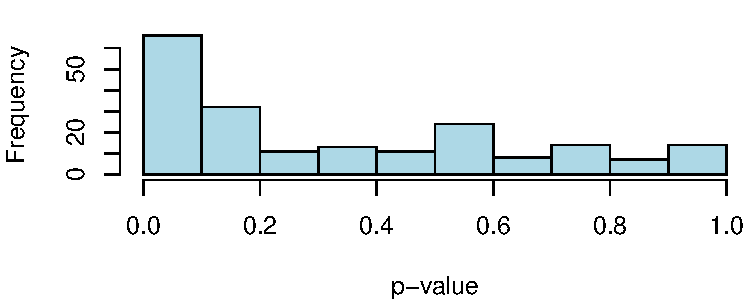
\includegraphics[width=4.1in]{graphs/SCpvals}

\vskip .25cm

{\gr Some are clustered at zero, the rest sprawl out to one.}\\

FDR of $q=0.1$ yields  $\alpha=0.0122$ p-value rejection cut-off. \\Implies 25 `significant', of which approx 22-23 are true signals.

\end{frame}


\begin{frame}


A {\it cut} model, using only these 25  signals,
has $R_{cut}^2 = 0.18$.  \\
This is much smaller than the full model's $R_{full}^2=0.56$.

\vskip .5cm
In-Sample (IS) $R^2$ {\it always} increases with more covariates.
\\ {\gr This is exactly what MLE $\bs{\hat\beta}$ is fit to maximize.}
\\ {\theme But how well does each model predict {\it new} data?}

\vskip .5cm
{ An out-of-sample (OOS) experiment}
\begin{itemize}
\item split the data into 10 random subsets {(`folds')}.
\item Do 10x: fit model $\bs{\hat\beta}$ using only 9/10 of data, 
\\ ~~~~~~~~~~~and record $R^2$ on the left-out subset. 
\end{itemize}
These OOS $R^2$ give us a sense of how well each \\model can predict
data that it has not already seen.
\end{frame}

\begin{frame}

We gain predictive accuracy by {\it dropping} variables.

\begin{center}\vspace{-.2cm}
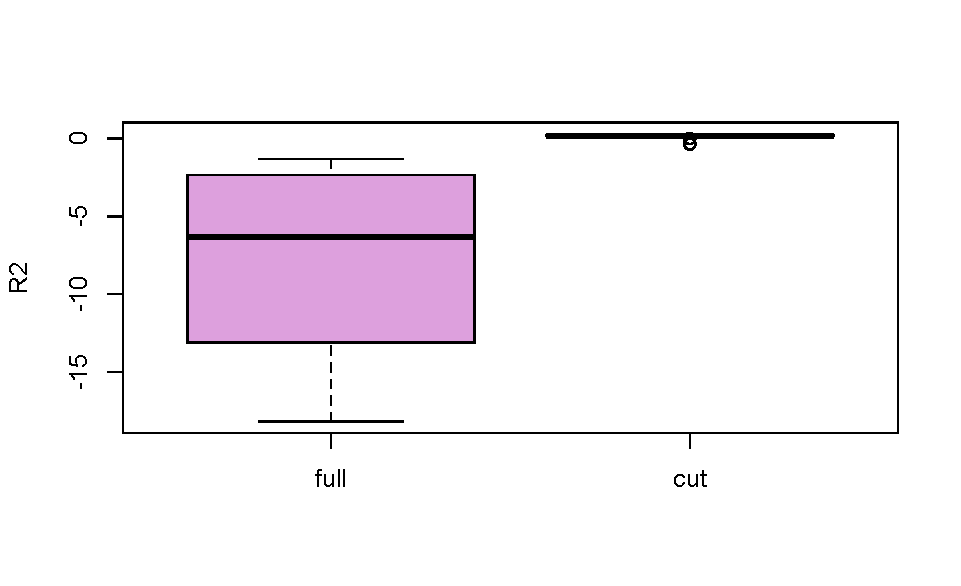
\includegraphics[width=4in]{graphs/SCr2}
\end{center}

Cut model has mean OOS R2 of 0.09, about 1/2 in-sample R2.

\vskip .2cm
The full model is terrible.  It is overfit and worse than $\bar y$.\\ 
{\nv Negative R2 are more common than you might expect.}

\vspace{-.2cm}
\end{frame}

\begin{frame}


{\nv All that matters is Out-of-Sample $R^2$.}  \\{\theme We don't care about In Sample $R^2$.}

\vskip .5cm
Using OOS experiments to  choose the best model is called {\it cross validation}.  It will be a big part of our big data lives.

\vskip .5cm
Selection of `the best' model is at the core of all big data.

\vskip .1cm
But before getting to selection, we first need strategies to \\ build good sets of candidate models to choose amongst.

\end{frame}



\begin{frame}

{\bf Regularization}

\vskip .5cm
The key to contemporary statistics is
{\nv regularization:} \\~~~~~~~~~~~~~~~depart from optimality to stabilize a system.

{\gr Common in engineering: I wouldn't drive on an optimal bridge.}

\vskip .5cm
We minimize deviance \onslide<2->{{\nv plus a cost on the size of
coefficients.}} {\large\begin{equation*}
\mr{min} 
-\frac{2}{n}\log \text{LHD}(\bs{\beta}) 
\onslide<2->{{\nv + \lambda\sum_k |\beta_k|}}
\end{equation*}}

\vskip -.25cm
\onslide<2>{This particular cost gives the `lasso': the new least squares.}

\end{frame}


\begin{frame}

{\bf Decision theory: \theme Cost in Estimation}

\vskip .5cm
Decision theory is based on the idea that choices have costs.\\
Estimation and hypothesis testing: what are the costs?


\vskip .5cm 
{\nv Estimation:}

\vskip .1cm
Deviance is the cost of distance between data and the model.\\
{\gr Recall: $\sum_i (y_i-\hat{y}_i)^2$ or 
$-\sum_i y_i\log(\hat{p}_i) - (1-y_i )\log(1-\hat{p}_i)$.}

\vskip .25cm
{\nv Testing:}

\vskip .1cm
Since $\hat{\beta}_j = 0$ is  {\it safe},  it should cost us to
decide otherwise.

\vskip .5cm 
$\Rightarrow$ The cost of $\hat{\beta}$ is deviance plus
a penalty  away from zero.



\end{frame}


\begin{frame}

{\bf{\gr [Sparse]}  Regularized Regression}


{\nv\large\[
\mr{min} \left\{ -\frac{2}{n}\log\text{LHD}(\bs{\beta}) + \lambda \sum_j c(\beta_j)\right\}
\]}

$\lambda >0$ is the penalty weight, $c$ is a cost (penalty) function.

$c(\beta)$ will be lowest at $\beta=0$ and we pay more for $|\beta| > 0$.

\vskip .1cm
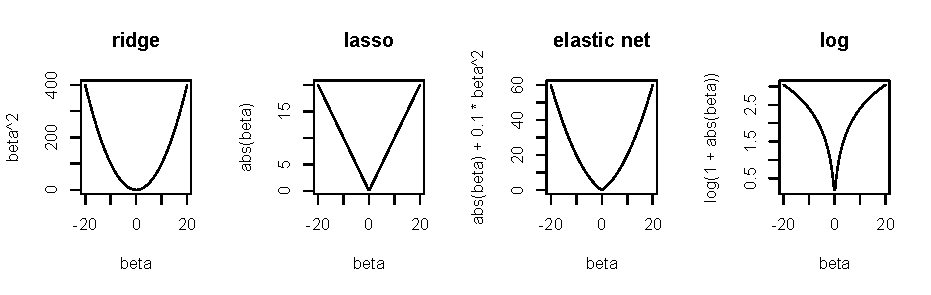
\includegraphics[width=4.25in]{graphs/penalties}

Options: ridge $\beta^2$, lasso $|\beta|$, elastic net $\alpha\beta^2 + |\beta|$,  $\log(1 + |\beta|)$.


\end{frame}


\begin{frame}

{\bf Penalization can yield {\theme automatic variable selection}}

The minimum of a smooth + pointy function can be at the point.

\vskip -.25cm
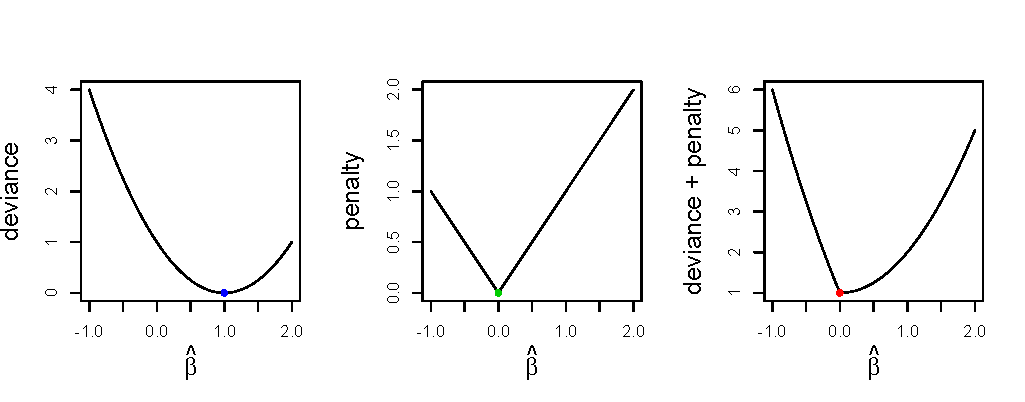
\includegraphics[width=4.25in]{graphs/penlasso}

\vskip .5cm
Anything with an absolute value (e.g., lasso) will do this.  

\vskip .1cm 
{\gr There are MANY penalty options and far too much theory.}

\vskip .1cm 
Think of lasso as a baseline, and others as variations on it.

\end{frame}

\begin{frame}

{\bf Lasso Regularization Paths}
\vskip .5cm

The lasso fits $\bs{\hat\beta}$ to minimize $-\frac{2}{n}\log\text{LHD}(\bs{\beta}) + \lambda \sum_j |\beta_j|$.

\vskip .1cm
We'll do this for a {\it sequence} of penalties $\lambda_1 > \lambda_2 ... > \lambda_T$.

\vskip .1cm
{\gr Then we can apply model selection tools to choose best $\hat \lambda$.}

\vskip .5cm
{\nv Path estimation:}

\vskip .1cm
~~~ Start with big $\lambda_1$ so big that $\bs{\hat \beta}=\bm{0}$.

\vskip .1cm
~~~ For $t=2\ldots T$: update $\bs{\hat \beta}$ to be optimal under $\lambda_t < \lambda_{t-1}$.

\vskip .5cm


Since estimated $\bs{\hat\beta}$ changes smoothly along this path:
\begin{itemize}
\item It's fast!  Each update is easy.
\item It's stable: optimal $\lambda_t$ may change a bit from sample to sample, but that won't affect the model much.
\end{itemize}

\end{frame}


\begin{frame}

The whole enterprise is easiest to understand visually.

\vskip -.25cm
\begin{center}
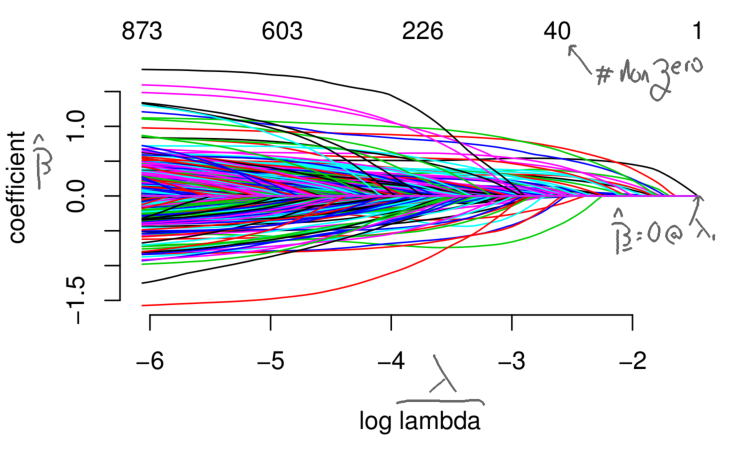
\includegraphics[width=.95\textwidth]{graphs/comscore_markeduppaths}
\end{center}

\vskip -.25cm
The algorithm moves {\it right to left}.  \\The $y$-axis is $\bs{\hat\beta}$ (each line a different $\hat\beta_j$) as a function of $\lambda_t$.
\end{frame}



\begin{frame}\

{\bf {\nv Example: } web browser data}

\vskip .5cm
The previous plot is  household log-online-spend regressed onto $\%$ of time spent on various websites (each $\beta_j$  a different site).

\vskip .25cm
Browsing and purchasing behavior for households:

\vskip .05cm
~I've extracted 2006 data for the 1000 most heavily trafficked \\~websites and for 10,000 households that spent at least 1\$.  


\vskip .25cm
Why do we care?  {\theme Predict consumption from browser history.}


\vskip .5cm
{\sf\nv faculty.chicagobooth.edu/matt.taddy/teaching/comscore.R}
\end{frame}


\begin{frame}


There are many packages for fitting lasso regressions in R.

\vskip .25cm
{\tt \nv glmnet} is most common.  {\tt \nv gamlr} is my contribution.

These two are very similar, and they share syntax.

\vskip .25cm
Big difference is what they do beyond a simple lasso:.

~~~{\tt\nv glmnet} does an `elastic net':  $c(\beta) = |\beta| + \nu \beta^2$.

~~~{\tt\nv gamlr} does  a `gamma lasso': $c(\beta) \approx \log(\nu + |\beta|)$.

\vskip .5cm  
Both use the {\tt \nv Matrix} library representation for {\theme sparse matrices}.
\end{frame}

\begin{frame}

A little bit more info on {\tt\nv gamlr}: \\ ~~~it actually applies a {\theme weighted}
$L_1$ penalty: $\lambda \sum_j \omega_j |\beta_j|$.  

\vskip .25cm
These weights {\theme adapt} along the regularization path as a function of the previous segment's solution
\begin{equation}\label{gammalasso}
\omega^{t}_j  = \left(1 + \gamma |\hat\beta^{t-1}_j|\right)^{-1} ~~j=1\ldots p 
\end{equation}
This lets you measure {\theme large signals with less bias}.

\vskip .25cm
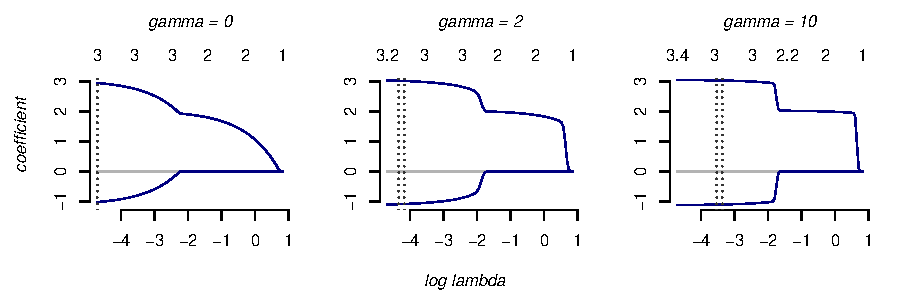
\includegraphics[width=\textwidth]{graphs/gamlr_eg}


\hfill See {\it Paths of One-Step Estimators} on my website.
\vskip -.2cm
 \end{frame}


\begin{frame}

{\bf Regularization and Selection}
\vskip .5cm


{The  lasso minimizes $-\frac{2}{n}\log\text{LHD}(\bs{\beta}) + \lambda \sum_j |\beta_j|$.}

\vskip .1cm
This `sparse regularization' auto-selects the variables.  

\vskip .1cm
{Sound too good to be true?  You need to choose $\lambda$.}

\vskip .5cm
Think of $\lambda>0$ as a signal-to-noise filter: {\it like squelch on a radio.}



\vskip .5cm We'll  use {\theme cross validation} or {\nv information criteria} to choose.


\vskip .5cm
Path algorithms are key to the whole framework:

\vskip .1cm
$\star$ They let us quickly enumerate a set of candidate models.

$\star$ This set is stable, so selected `best' is probably pretty good.

\end{frame}

\begin{frame}

A recipe for model selection.
\begin{enumerate}\bk
\item Find a manageable set of candidate models \\{(i.e., such that fitting all models is fast).}
\item Choose amongst these candidates the one with\\ best
predictive performance {\it on unseen data}.
\end{enumerate}

\vskip .5cm
{\nv 1.} is what the lasso paths provide.

\vskip .1cm
{\nv 2.} Seems impossible!  But it's not $\ldots$

\vskip .5cm 
First, define {\nv predictive performance} via `deviance'. 

\vskip .1cm
Then, we need to {\it estimate} deviance for a fitted model applied to {\it new independent observations} from the true data distribution.

\end{frame}


\begin{frame}
{\theme $\bs{K}$-fold Cross Validation}

\vskip -.3in
\hfill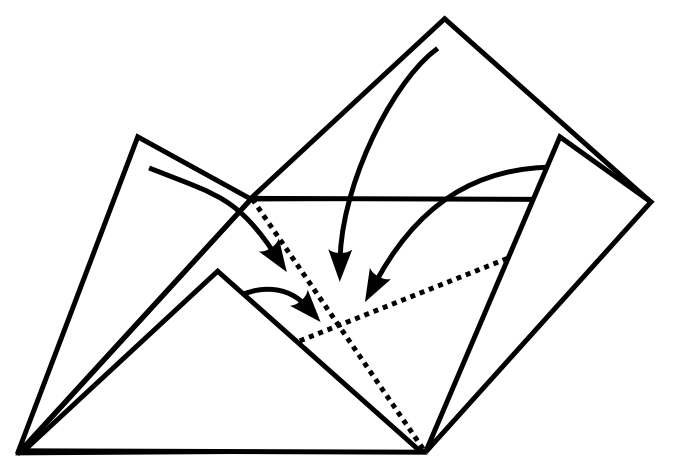
\includegraphics[width=2in]{graphs/fold}

\vskip -.9in {\gr One option is to just take \\repeated random samples.
\\
It is better to `fold' your data.}

\vskip 1cm
$\bullet$ Sample a random ordering of the data \\ { ~~(important to avoid order dependence)}

\vskip .1cm $\bullet$ Split the data into $K$ folds: { 1st 100/K\%, 2nd 100/K\%, etc}.

\vskip .1cm 
$\bullet$ Cycle through $K$ CV iterations with a single fold left-out.

\vskip .25cm
This guarantees each observation is left-out for validation, \\and lowers the sampling variance of CV model selection.

\vskip .25cm
Leave-one-out CV, with $K=n$, is nice but takes a long time.\\
$K=5$ to $10$ is fine in most applications.

\end{frame}


\begin{frame}
{CV Lasso}

The lasso path algorithm minimizes $-\frac{2}{n}\log\text{LHD}(\bs{\beta}) + \lambda_t \sum_j |\beta_j|$ over the sequence of penalty weights $\lambda_1 > \lambda_2 \ldots > \lambda_T$.

\vskip .25cm
This gives us a path of $T$ fitted coefficient vectors, 
$\nv \bs{\hat\beta}_1 \ldots \bs{\hat\beta}_T$,
each defining deviance for new data: $\nv -\log \text{p}(\bm{y}^{new}\mid\bm{X}^{new}\bs{\hat\beta}_t)$.

\vskip .5cm
Set a sequence of penalties $\lambda_1 \ldots \lambda_T$.  \\
Then, for each of $k=1\ldots K$ folds,
\begin{itemize}
\item Fit the path $\nv \bs{\hat\beta}^k_1 \ldots \bs{\hat\beta}^k_T$ on all data {\it except} fold $k$.
\item Get fitted deviance {\it on left-out data}: 
$\nv -\log \text{p}(\bm{y}^{k}\mid\bm{X}^{k}\bs{\hat\beta}_t)$.
\end{itemize}

This gives us $K$ draws of OOS deviance for each $\lambda_t$.

\vskip .5cm
Finally, use the results to choose the `best' $\theme \hat\lambda$, then re-fit the model to {\it all of the data} 
by minimizing $-\frac{2}{n}\log\text{LHD}(\bs{\beta}) 
+ {\theme \hat \lambda} \sum_j |\beta_j|$.

\end{frame}


\begin{frame}[fragile]
{CV Lasso}

{Both {\tt gamlr} and {\tt glmnet} have functions to wrap this all up.}

The syntax is the same; just preface with {\tt cv.}

\begin{semiverbatim}\nv
cv.spender <- cv.gamlr(xweb, log(yspend))
\end{semiverbatim}

Then, {\nv\tt coef(cv.spender)} gives you $\bs{\hat\beta}_t$ at the `best' $\lambda_t$
\begin{itemize}
\item {\tt select="min"} gives $\lambda_t$ with {\it min average OOS deviance}.
\item {\tt select="1se"} defines best as {\it biggest $\lambda_t$ with average OOS deviance no more than 1SD away from the minimum.}
\end{itemize}

\vskip .2cm
{\tt 1se} is default, and balances prediction against false discovery.  

{\tt min} is purely focused on predictive performance.

\end{frame}


\begin{frame}
{CV Lasso}

\vskip .25cm

Again, the routine is most easily understood visually.

\vskip -.25cm
\begin{center}
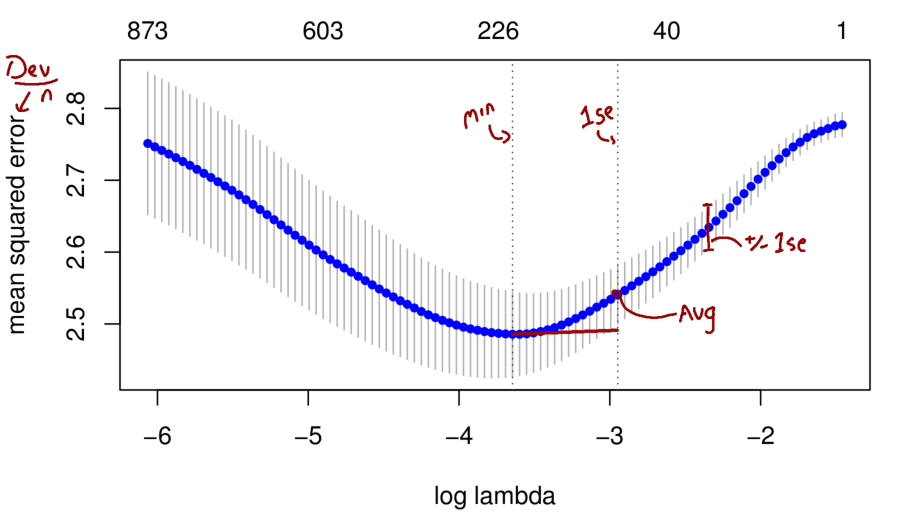
\includegraphics[width=\textwidth]{graphs/comscore_cvmarkedup}
\end{center}

\vskip -.25cm
Both selection rules are good; {\tt 1se} has extra bias for simplicity.
\end{frame}

\begin{frame}
{Problems with Cross Validation}

\vskip .5cm \nv It is time consuming:
{\bk When estimation is not instant, \\
fitting $K$ times can become unfeasible even $K$ in 5-10. }

\vskip .5cm It can be unstable: {\bk imagine doing CV on many different samples.  
There can be large variability on the model chosen.}

\vskip .5cm It is hard not to cheat: {\bk for example, with the FDR cut model we've
already used the full $n$ observations to  select the 25 strongest
variables.  It is not surprising they do well `OOS'.}

{\gr The rules: if you do something to the data, do it {\it inside} CV.}

\vskip .5cm \bk Still, some form of CV is used in most DM applications.
\end{frame}



\begin{frame}[fragile]

{
\bf \gr Alternatives to CV: \bk Information Criteria}

\vskip .25cm
{Many `Information Criteria' out there: AICc, AIC, BIC, ...}

These approximate distance between a model and `the truth'.

You can apply them by choosing the model with minimum IC.

\vskip .5cm
Most common is Akaike's {\theme AIC = Deviance + $2df$.}

\vskip .2cm
$df$ = `degrees of freedom' used in your model fit.

For lasso and MLE, this is just the $\#$ of nonzero $\hat\beta_j$.

\end{frame}

\begin{frame}
{AIC overfits in high dimensions}

The AIC is atually estimating OOS deviance: 
what your deviance would be on another {\it independent} sample of size $n$.

\vskip .5cm
IS deviance is too small, since the model is tuned to this data.  \\Some deep theory shows that IS - OOS deviance $\approx 2df$.
\vskip .1cm

\hskip 2in $\Rightarrow \text{AIC} \approx$ OOS deviance.

\vskip .5cm
Its common to claim this approx (i.e., AIC) is good for `big $n$'.

{\theme Actually, its only good for big $n/df$. } 

\vskip .5cm
In Big Data, $df$ (\# parameters) can be huge.  Often $df\approx n$.

In this case the AIC will be a bad approximation: it overfits!

\end{frame}

\begin{frame}
{AIC corrected: \nv AICc}

AIC approximates OOS deviance, but does a bad job for big $df$.
 
\vskip .5cm
In linear regression an improved approx to OOS deviance is
\[
\theme \text{AICc} { ~\gr = \text{Deviance} + 2df\ds{E}\left[\frac{\sigma^2}{\hat \sigma^2}\right]} = \text{Deviance} + 2df\frac{n}{n-df-1}
\]
This is the corrected AIC, or AICc.  

\vskip .05cm
{It also works nicely in logistic regression, or for any {\tt glm}.}

\vskip .5cm
Notice that for big $n/df$, AICc $\approx$ AIC. So {\it always} use AICc.

\end{frame}

\begin{frame}[fragile]
{gamlr uses AICc}

\vskip .25cm

{It's marked on the path plot}

\vskip .25cm
\hskip .5in 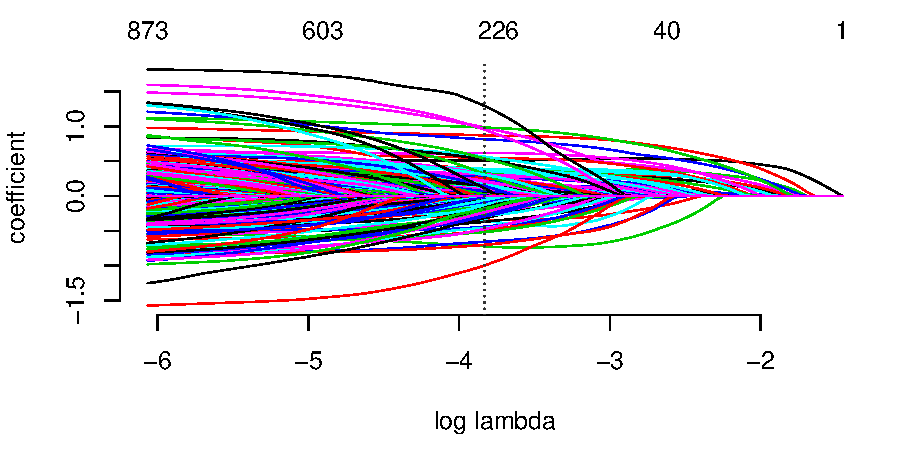
\includegraphics[width=.8\textwidth]{graphs/comscore_pathaicc}

\vskip .1cm
And it is the default for {\tt coef.gamlr}

\begin{semiverbatim}\nv\small
B <- coef(spender)[-1,] 
B[c(which.min(B),which.max(B))]\bk
    cursormania.com shopyourbargain.com 
          -0.998143            1.294246 
\end{semiverbatim}

\end{frame}


\begin{frame}
{IC and CV on the Comscore Data}

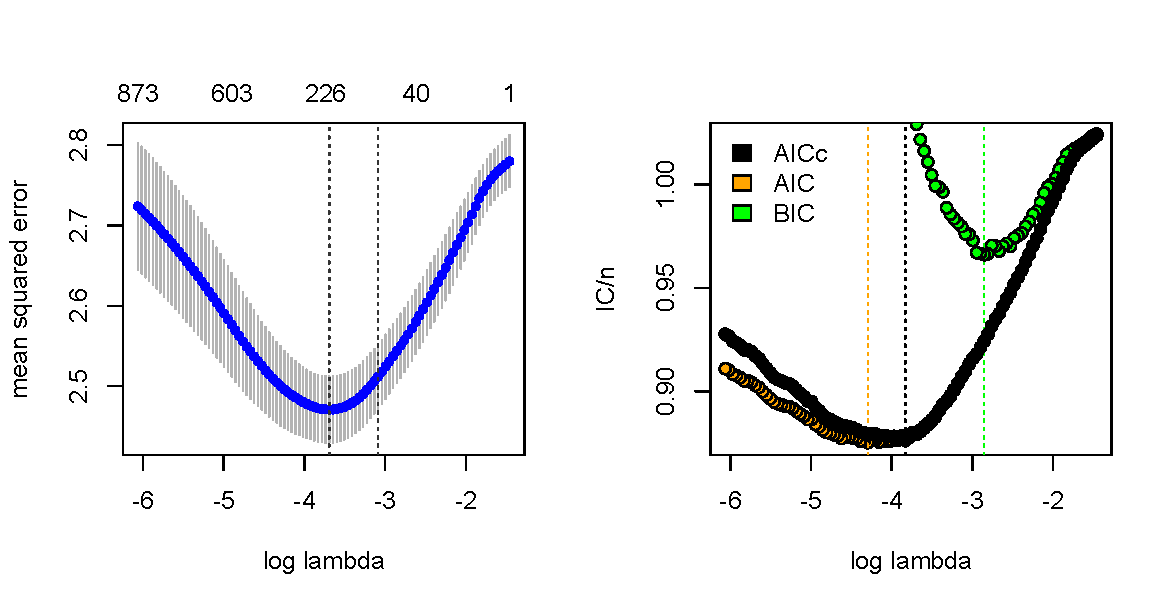
\includegraphics[width=\textwidth]{graphs/comscore_icvcv}

\vskip .5cm
The take home message: AICc curve looks like CV curve.

 \vskip .25cm
In practice, BIC works more like the 1se CV rule.  \\
But with big $n$ it chooses too simple models (it underfits).

\end{frame}


\begin{frame}
{IC and CV on the Comscore Data}

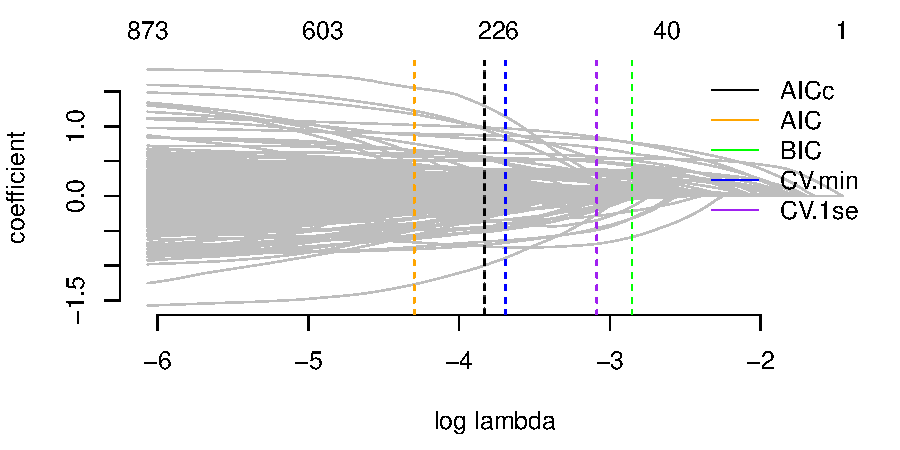
\includegraphics[width=\textwidth]{graphs/comscore_pathallic}

\vskip .2cm
With all of these selection rules, you get a range of answers.

If you have time, do CV.  But AICc is fast and stable.

If you are worried about false discovery, tend towards BIC/1se.

\end{frame}


\begin{frame}
{Causal Inference}

We've used {\it prediction} as a basis for model building: 

\vskip .1cm
~~{\nv choose a fitting
routine to do the best job forecasting $y$ at \\~~new $\bm{x}$ drawn from the same
distribution as data sample $\bm{X}$.}

\vskip .1cm
{ This exactly the question tackled by CV and AICc. }

\vskip .5cm
Now, we'll try to estimate the effect of a special covariate:

\vskip .1cm
 {\theme ~~Treatment `$d$', which we can change {\it independently} from $\bm{x}$.}

\vskip .1cm
That is: we want to know the causal {\it treatment effect} (TE).

\vskip .25cm
{For example,
\begin{itemize}
\item $d=1$ if you get the drug, $d=0$ for placebo (control).
\item $d$ is some {\it policy tool}, like interest rates or product price.
\end{itemize}}

\end{frame}


\begin{frame}
{ Observational Studies}

Our treatment effect (TE) model looks like
\[
\ds{E}[y|d,\bm{x}] = \alpha + d\gamma + \bm{x}'\bs{\beta}
\]
and we'll want to interpret the estimated {\it treatment effect} $\hat \gamma$  as change in $y$ when $d$ moves {\theme independent} of all other influencers.

\vskip .5cm
This is easy to measure in a fully randomized experiment, \\because $d$ is independent by design: we sample it randomly.

\vskip .5cm
Without an experiment, we need to {\theme control for}  (i.e., remove from $\hat\gamma$) all influences on $y$ which are correlated with $d$.


\vskip .25cm
These other influencers are called {\nv confounders}.\\
We  control for them by {\nv including them in regression.}


\end{frame}

\begin{frame}

How does controlling for confounders work?

\vskip .2cm
With  $\bm{x}$ in the regression model, inference for $\gamma$ is measured from the effect of {\it the bit of $\bm{d}$ that is not predictable by $\bm{x}$.}

\vskip .5cm
e.g., say $\theme d(\bm{x}) =\bm{x}'\bs{\tau} + \nu$, where $\nu$ is random noise (residual).
\begin{align*}
\text{Then:~~~~}~\ds{E}[y|\bm{x},d] & = {\theme d\gamma} + \bm{x}'\bs{\beta}\\
& =  {\theme (\bm{x}'\bs{\tau} + \nu)\gamma} + \bm{x}'\bs{\beta}\\
& = {\theme\nu\gamma} + \bm{x}'(\gamma\bs{\tau}+\bs{\beta}) \gr \approx 
\nu\hat\gamma + \bm{x}'\bs{\hat\beta}
\end{align*}

So $\hat\gamma$ is {\it identified} as the effect of $\nu$, the independent part of $d$.

\vskip .5cm
This type of controlling is simple with low-D $\bm{x}$: just fit the MLE regression and your standard errors on $\hat\gamma$ should be correct.

{\theme But this fails if you have too many controls.}

\end{frame}


\begin{frame}
{Multicollinearity and the lasso}


{\it Can't we just throw everything in a lasso?}

\vskip .2cm
Not exactly.  

\vskip .2cm
Even if all possible influencers are in $\bm{x}$, the lasso won't always choose the right ones to remove confounding effects.

\vskip .5cm
In the previous slide's example, we could have also \\written $\bm{x} = \bs{\varphi}d + \upsilon$, so that $\bm{x}$ is now a function of $d$.
\begin{align*}
\text{Then:~~~~}~\ds{E}[y|\bm{x},d] & = d\gamma + \bm{x}'\bs{\beta} =  d(\gamma + \bs{\varphi}'\bs{\beta}) + \upsilon \bs{\beta}
\end{align*}
Since the lasso makes you pay a price for every extra nonzero coefficient, it'll choose to just collapse the effects of $\bm{x}$  ($\bs{\beta}$) into $\hat\gamma$ \\
{\gr (unless $\upsilon$ has a big enough effect to warrant the extra cost.)}

\end{frame}


\begin{frame}

{\bf Causal Lassos}

\vskip .25cm
Recall how we started today: we want to reduce dimension in the directions that are relevant to our decision making.

\vskip .25cm
The problem is that $d = d(\bm{x}) + \nu$, and {\nv  we want the effect of $\nu$}.

\vskip .1cm
{So estimate $\hat d(\bm{x})$ directly and include it in the regression!}

\vskip .5cm
Any left over effect of $d$ will be attributable to $d-\hat d(\bm{x}) = \nu$.
\[
\ds{E}[y|\bm{x}] = {\theme (\hat d(\bm{x}) + \nu)\gamma} + \hat d(\bm{x})\delta +
\bm{x}'\bs{\beta} = {\theme \nu\gamma} + \hat d(\bm{x})(\gamma+\delta) +
\bm{x}'\bs{\beta}
\]


Controlling for $\hat d(\bm{x})$ in regression is equivalent\\ to estimating $\hat\gamma$ as the effect of $\nu$: {\it the independent part of $d$}. 

\end{frame}

\begin{frame}
{A Treatment Effects Lasso}

Two stages:
\begin{enumerate}
\item Estimate $\hat d(\bm{x})$ with lasso regression of $d$ on $\bm{x}$.
\item Do a lasso of $y$ on [$d$, $\hat d(\bm{x})$, $\bm{x}$], with $\hat d(\bm{x})$ {\it unpenalized}.
\end{enumerate}

\vskip .25cm
Including $\hat d$ unpenalized in [2] ensures that  confounder effects on $d$ have been removed: thus $\hat\gamma$ measures the effect of $\nu$.

\vskip .25cm
In [2], we can apply our usual AICc lasso to see \\what else in $\bm{x}$ effects $y$ and, most importantly, if $\hat\gamma \neq 0$.

\vskip .25cm
We've replaced causal estimation with two prediction problems.

And prediction is something we're really good at, even in HD.


\vskip .25cm
{\theme In the end, we're asking: is $\nu$ {\it useful} for predicting $y$?}

\end{frame}


\begin{frame}
{ Freakonomics: \theme Abortion and Crime}

\begin{columns}

\column{2in}

\vskip .5cm
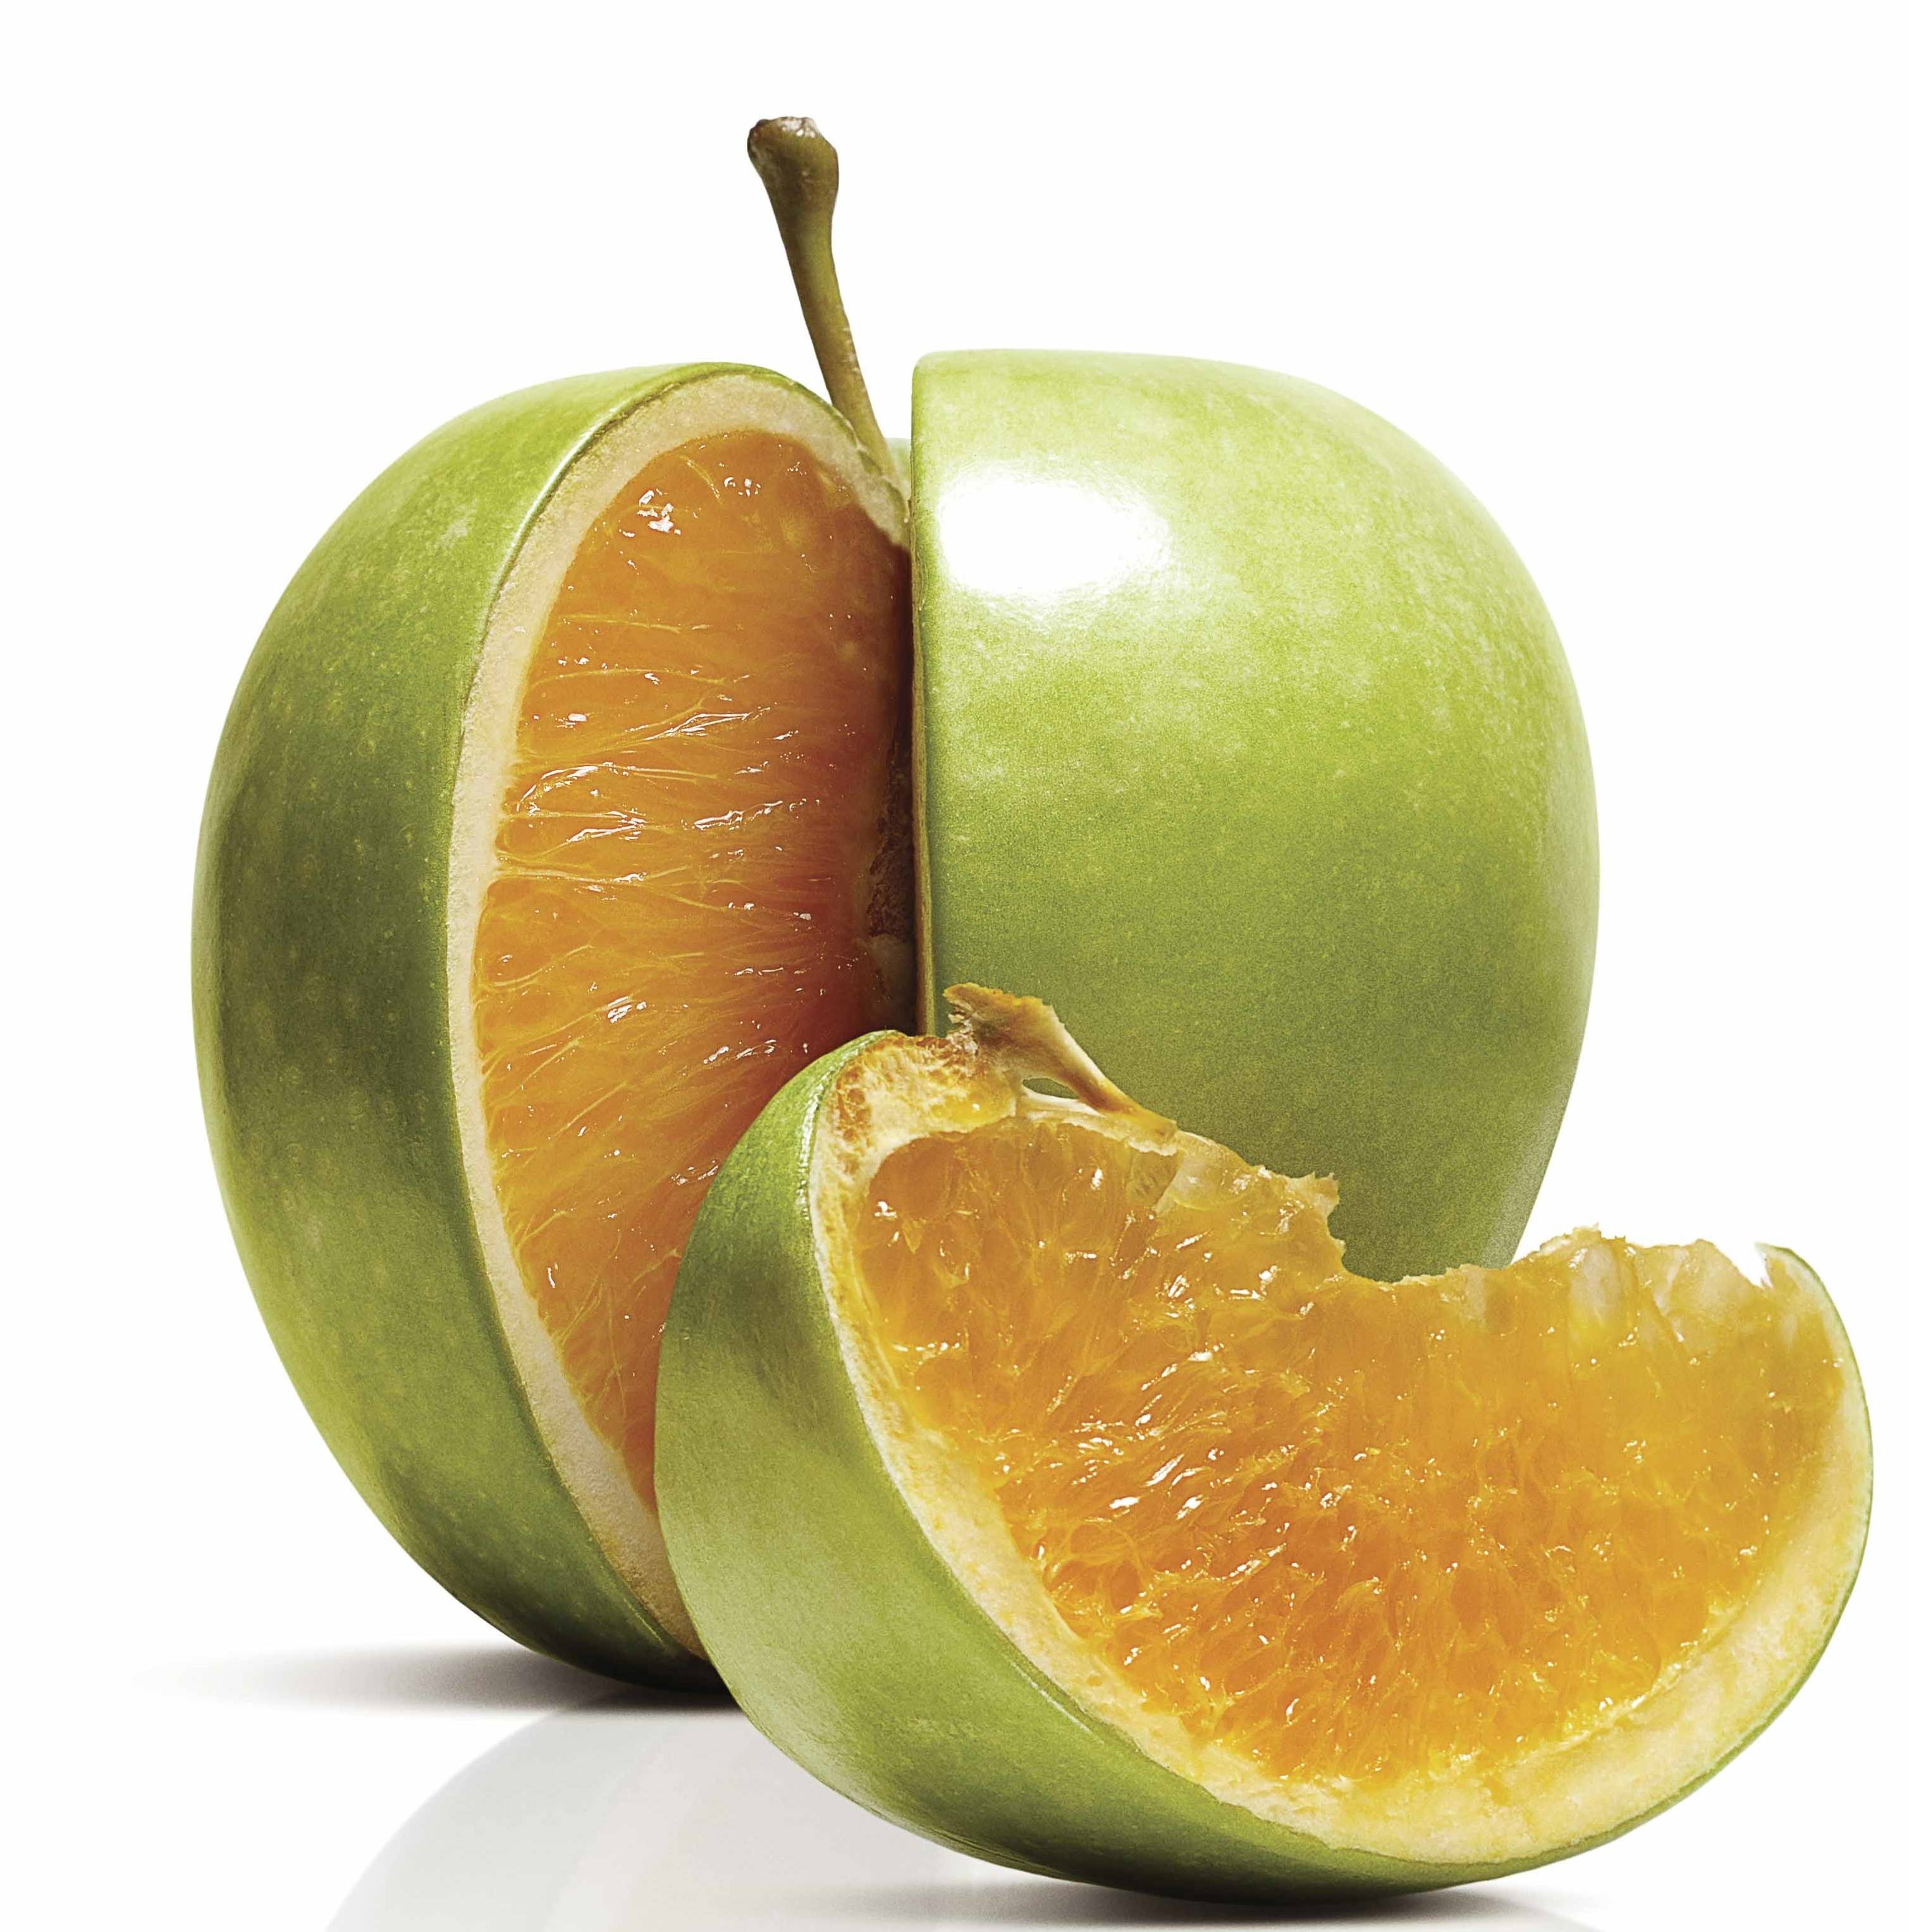
\includegraphics[width=2in]{graphs/apple-orange}

\column{2in}



\vskip .25cm
Donahoe and Levitt (DL) argue a controversial thesis:

\vskip .1cm{\nv
\hfill easier access to abortion \\\hfill{\it causes} decreased crime.}

\vskip .25cm Proposed mechanism holds that birth is  postponed until the
mother is more ready.

\end{columns}

\vskip .5cm
{They assume stable family $\Rightarrow$ better upbringing $\Rightarrow$ less crime.}

\vskip .5cm
There's obviously no experiment here.  \\How have they controlled for confounders?

\end{frame}

\begin{frame}[fragile]
{Crime $\sim$ Abortion regression}

{The treatment variable $d$ is by-state abortion rate, \\
and for response we look at {\theme $y=$ murder rate}.}

\vskip .25cm
DL {\it control} for bunch of state-specific {\it confounders}: income, poverty, child tax credits, weapons laws, beer consumption... 

\vskip .2cm
They also include state effects {\gr (factor `$s$')} and a time trend {\gr (numeric `$t$'')} to control for missed confounders.

{\nv \footnotesize
\begin{semiverbatim}
> orig = glm(y ~ d + t + s + ., data=controls) 
> summary(orig)\$coef[`d',]\bk
     Estimate    Std. Error       t value      Pr(>|t|) 
-2.098119e-01  4.109177e-02 -5.105936e+00  4.505925e-07 
\end{semiverbatim}}

{\theme Abortion has a very significant effect!}
Skeptical?  You should be.
\end{frame}



\begin{frame}
{Alternative story: \theme Cellphones and Murder}

{Technology has contributed to
lower murder rates, and we'll add cellphone
subscribers as a variable to control for tech progress.}

\vskip .1cm

{\gr   e.g., Cellphones lead to faster 
ambulances, our jobs are  gentile so we're 
less rough, more communication increases empathy, 
or we don't interact in-person
because we don't have to.}

\vskip .25cm
~~~~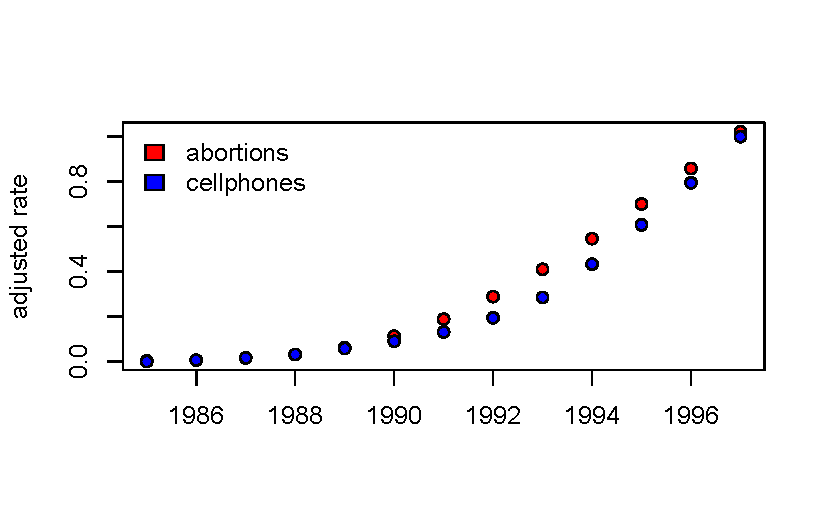
\includegraphics[width=3.75in]{graphs/cellphone_abortions}

Abortion and cellphones move together...

\vskip -.4cm
\end{frame}

\begin{frame}[fragile]

{\nv \footnotesize
\begin{semiverbatim}
> tech = glm(y ~ phone + t + s + ., data=controls)
> summary(tech)\$coef[c(`phone'),]\bk
     Estimate    Std. Error       t value      Pr(>|t|) 
-3.662545e-01  6.779352e-02 -5.402500e+00  9.699480e-08 
\end{semiverbatim}}

\vskip -.25cm
{\theme \hfill Cellphones have an even more significant effect!}


\vskip .5cm
It took me about 10 minutes to dream up a\\ causal variable and grab data off of wikipedia.  

\vskip .5cm What is happening is that murder decreased quadratically,\\
and we have no controls that also moved this way.

\vskip .5cm
How can we be sure the abortion effect is not just a stand-in
for another cause that changed quadratically over the years?\\


\end{frame}


\begin{frame}[fragile]

To {\it control} for such confounders, we just add {\theme $t^2$} to the model.

\vskip .2cm
We should also allow confounder effects to interact with each other
(e.g., different {\tt gun} effect for high {\tt beer}) and with time.

\vskip .25cm
But now we've added so many variables that there is not enough data to say anything.

{\nv \footnotesize\vspace{-.25cm}
\begin{semiverbatim}
> dim(model.matrix(y ~ d + (s + .^2)*(t+t2), data=cntrls))
\bk [1] 624 280
\end{semiverbatim}}


We can't expect to fully control for every crazy story.\\
We'd like to select amongst HD controls those we really need.

\vskip .25cm
\hfill \theme $\Rightarrow$ Use the double lassos to first control, then estimate.
\end{frame}


\begin{frame}[fragile]


{AICc lasso selects $d$ as highly predicted by $\bm{x}$.}

~~~~~~~~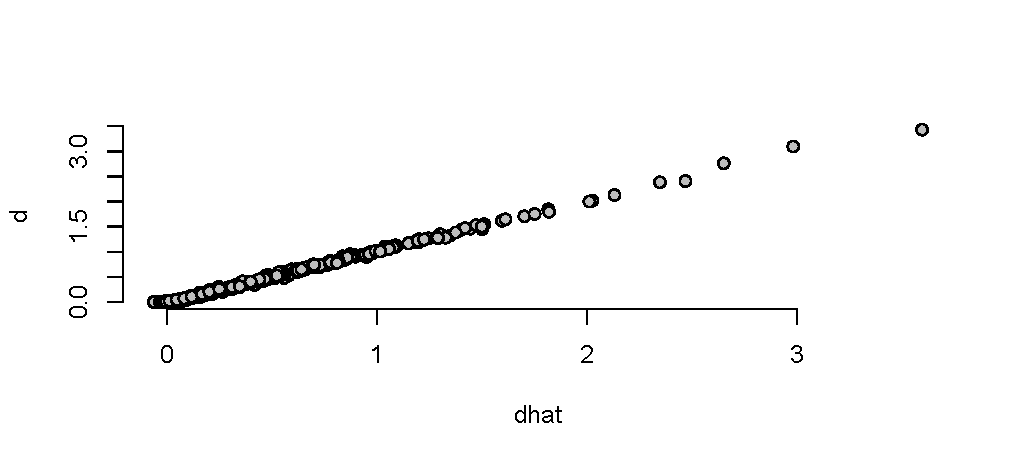
\includegraphics[width=3.5in]{graphs/AbortionDhat}


There's almost no {\it independent} movement of abortion rates to measure as effecting crime (it's not much of an experiment).

\vskip .25cm
{Sure enough, if you include {\tt dhat} in lasso regression \\then AICc says there is no residual effect for $d$.}

\begin{semiverbatim}\gr
## free=2 here leaves dhat unpenalized\nv
> causal <- gamlr(cBind(d,dhat,x),y,free=2)
> coef(causal)["d",] \bk
[1] 0
\end{semiverbatim}

\vskip -.5cm
\end{frame}


\end{document}






























